

\section{Размытая разрывная регрессия}



\begin{frame}{Пример: оценка спроса на образование в Нью-Йорке} % НУЖЕН ЕЩЕ ПРИМЕР С ТОЧНО БИНАРНЫМ T

\begin{figure}
    \centering
    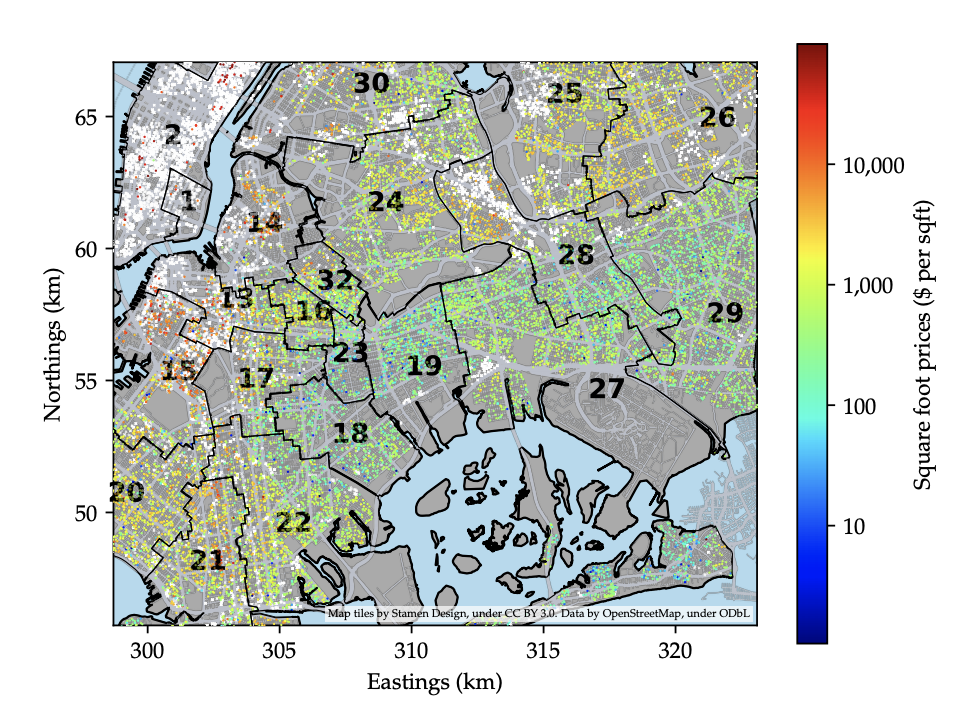
\includegraphics[width=0.9\textwidth]{Images/ny_schools_map.png}
\end{figure}

\end{frame}

\begin{frame}{Плацебо тест}


\begin{figure}
    \centering
    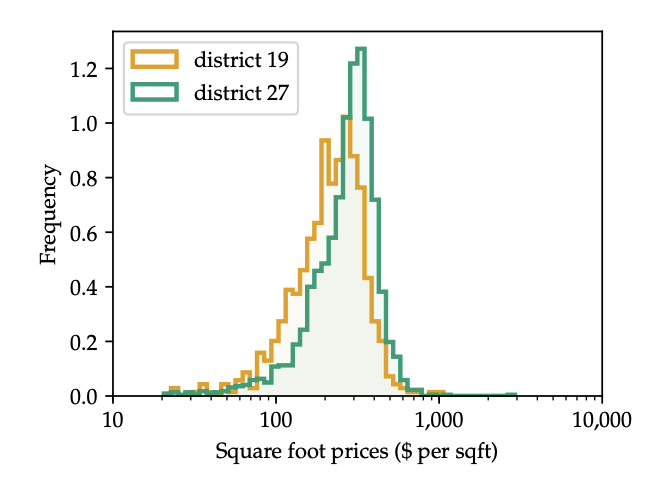
\includegraphics[width=\textwidth]{Images/placebo_schools_ny.png}
\end{figure}

\end{frame}


\begin{frame}{Fuzzy regression discontinuity}
\begin{figure}
    \centering
    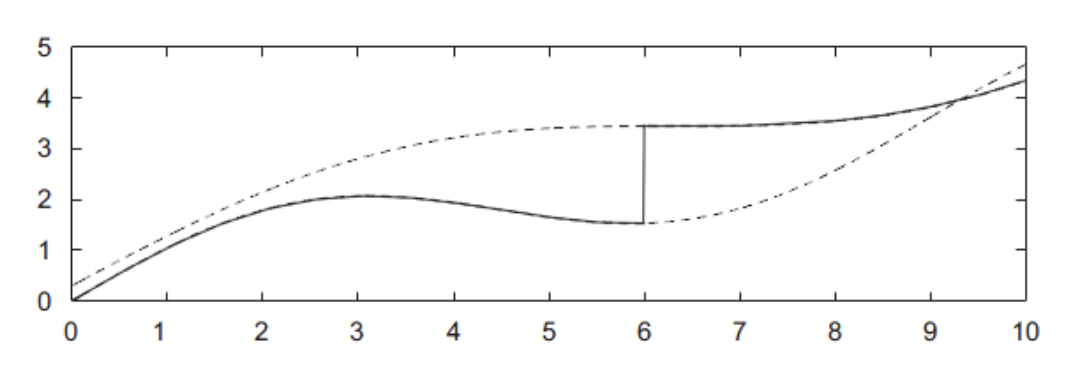
\includegraphics[width=\textwidth]{Images/sharp.png}
    \label{Sharp RDD}
\end{figure}
IV + Sharp RDD = Fuzzy RDD

\begin{figure}
    \centering
    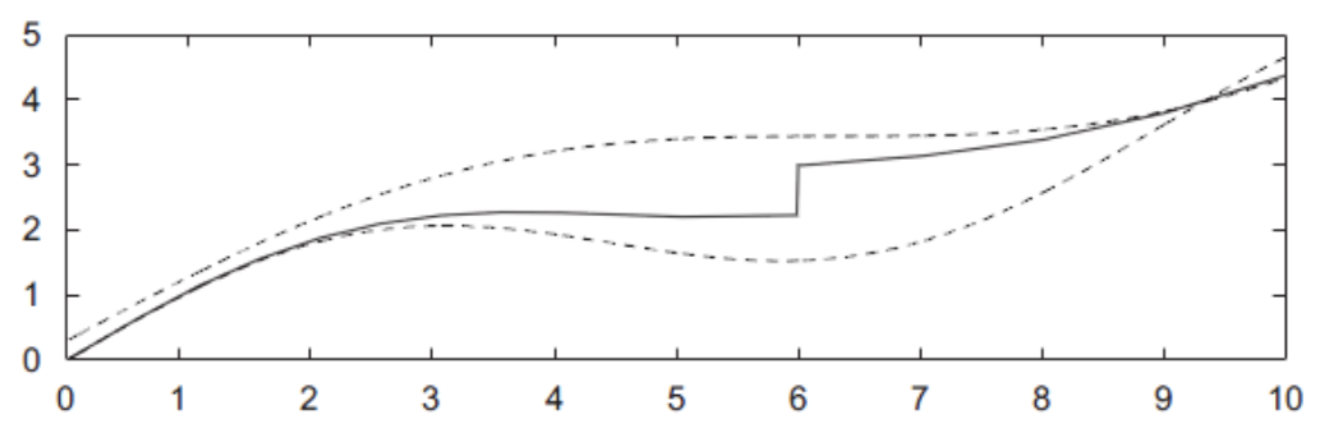
\includegraphics[width=\textwidth]{Images/fuzzy.png}
    \label{Fuzzy RDD}
\end{figure}
\end{frame}


\begin{frame}{Четкая разрывная регрессия: Предположения}
    \begin{figure}
    \centering
    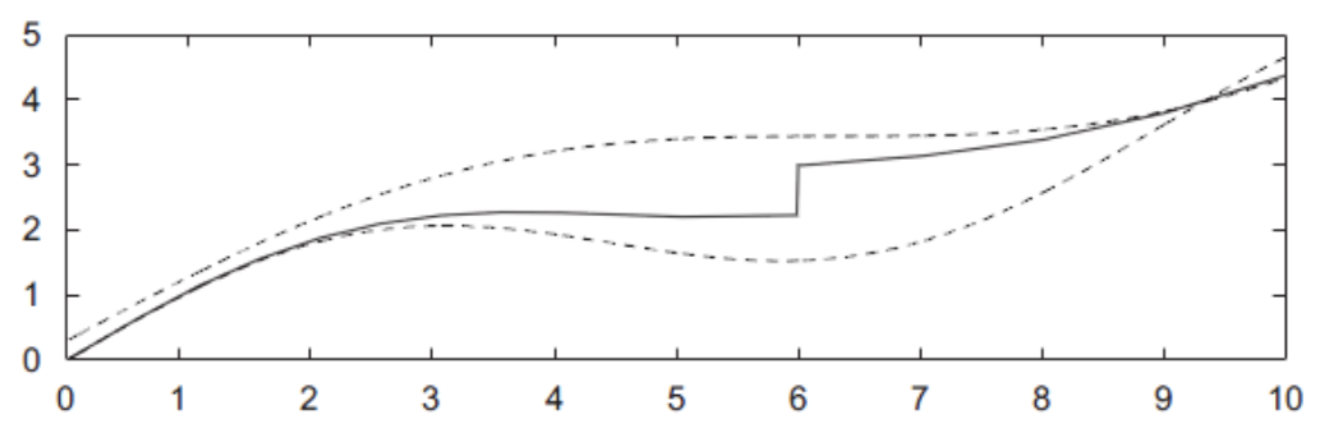
\includegraphics[width=\textwidth]{Images/fuzzy.png}
    \label{Fuzzy RDD}
\end{figure}
    \begin{itemize}
    \item Что у нас инстументальная переменная? \visible<2->{Z = R > c}
    \item Что у нас переменная интереса? \visible<3->{T}
    \item Главное предположение разрывной регрессии: \visible<4->{Предположим непрерывность всего: $E(Y_{00}|R), E(Y_{01}|R), E(Y_{10}|R), E(Y_{11}|R)$, $E(T_{0}|R), E(T_{1}|R), E(X|R)$}
    \end{itemize}
\end{frame}
